\documentclass[10pt, conference]{IEEEtran}
% \usepackage{silence}
% \WarningFilter[newline]{latex}{Underfull}

\usepackage{booktabs}
\usepackage{float}
\usepackage{multirow}

\usepackage{ifpdf}
% Enable correct encoding
\ifpdf{}
    \usepackage[utf8]{inputenc}
\fi{}
\usepackage[T1]{fontenc}

\usepackage[pdftex]{hyperref} % Enable hyperlinks
% \hypersetup{hidelinks}

% Citations Package
\usepackage[
    backend=biber,
    style=ieee
]{biblatex}
\addbibresource{citations.bib}

\title{Deep Learning’s Potential --- Differentiating Between Images of Concepts
and Tangible Objects}


\author{%
    \IEEEauthorblockN{Pratik Bhusal}
    \IEEEauthorblockA{%
        pratik.bhusal@utdallas.edu\\
        \today
    }\\

    \IEEEauthorblockN{Max Xie}
    \IEEEauthorblockA{%
        max.xie@utdallas.edu\\
        \today
    }
}

\usepackage{tabulary}
\usepackage{graphicx}
\usepackage{svg}


% 2. Report Presentation (40\%): % {{{


%     1. Is the format correct? IEEE two-column style format, with the font name Times
%     New Roman and size 10.

%     2. Are there obvious grammatical errors or incomplete sentences?

%     3. Are there required sections missing? Each report should include title,
%     abstract, introduction, related work, one or more technical sections, one
%     section about empirical analysis, conclusion, and references.

%     4. Does the report contain plagiarism content?

%     5. Is the proposed AI algorithms and/or models described in sufficient detail?

%     6. What is an overall evaluation of the presentation?

%     7. Is there a clear description about the feature extraction process? Are
%     the features clearly described?

% % }}}

% 3. Technical content (50%): {{{

%     1. Does the implementation code include plagiarism content?

%     2. Is the code uploaded?

%     3. Is there any exploratory data analysis?

%     4. Are the research problem and the main tasks clearly described? The
%     students in one team should focus on separate tasks. If some students
%     focused on the same tasks, the differences of their contributions should be
%     described clearly.

%     5. What is the overall level of efforts for the main tasks. Each report
%     should clearly describe which parts of the code were written by the author.
%     The load of coding can be measured by the the time that is required to
%     implement and debug the code. This time will be estimated by the instructor
%     and TA based on an overall evaluation of the code.  If the load of coding is
%     too low (e.g., 2 hours), the level of efforts will be low (e.g, 0.2). If the
%     load of coding is high (e.g., 50 hours), the level of efforts will be high
%     (e.g., 0.9).

%     6. What is the level of originality and creativity about the proposed work?

%         Examples of high originality and creativity are: (1) The proposed work
%         replicates the results of an existing paper and conducts some new
%         empirical analysis not reported in the paper, such as empirical analysis
%         based on new evaluation metrics (e.g., area under curve, area under
%         precision-recall curve) and new datasets not considered in the paper.
%         (2) The proposed work conducts an empirical comparison between the
%         methods proposed in several different papers. (3) The proposed work
%         develops new algorithms or new neural network architectures and
%         demonstrates the effectiveness and/or efficiency of the proposed
%         techniques, in comparison with some baseline methods in real-world
%         datasets. Algorithms and neural network architectures modified from
%         existing ones are also considered as new. (4) The proposed work presents
%         novel applications of AI models that have not been studied in the
%         current literature. (5) The proposed work develops new algorithms and/or
%         models for Kaggle competitions and demonstrates the effectiveness and/or
%         efficiency of the proposed techniques on the kaggle datasets, in
%         comparison with some baseline methods.

%         Examples of low/medium originality and creativity: (1) The proposed work
%         only replicates the results of an existing paper but does not conduct
%         any new empirical analysis. (2) The proposed work implements classic AI
%         models (e.g., logistic regression, linear regression, bayesian neural
%         networks, support vector machines) for classic problems (e.g.,
%         classification, regression) on some benchmark datasets.

% 7. Is there a detailed discussion about how the hyper parameters were turned?
% Have the finalized hyperparameters of all the AI models been reported?

% 8. Are the empirical results discussed in sufficient detail?

% % }}}

\begin{document}


\begin{figure}[H]
    \centering
    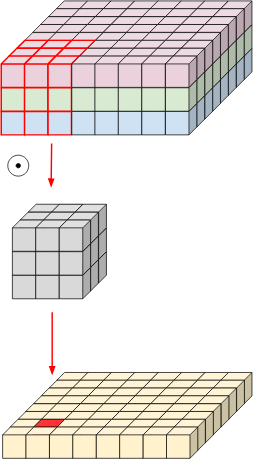
\includegraphics[height=50ex]{./figures/standardConvolution.png}
    \caption{Standard 2D Convolution~\cite{depthWiseConvolutionImages}}\label{fig:standard2DConvolution}
\end{figure}


\begin{figure}[H]
    \centering
    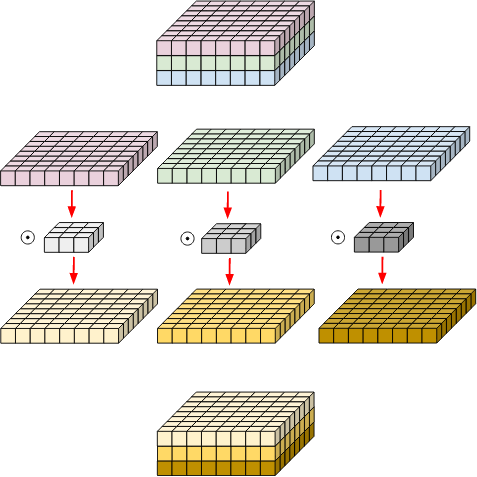
\includegraphics[height=50ex]{./figures/depthWiseConvolution.png}
    \caption{Depth-Wise Convolution~\cite{depthWiseConvolutionImages}}%
    \label{fig:depthWiseConvolution}
\end{figure}


\begin{figure}[H]
    \centering
    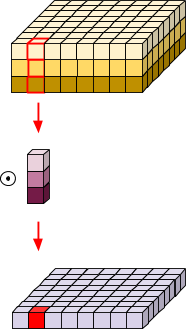
\includegraphics[height=50ex]{./figures/depthWiseSeparableConvolution.png}
    \caption{Depth-Wise Convolution~\cite{depthWiseConvolutionImages}}%
    \label{fig:depthWiseSeparableConvolution}
\end{figure}

\begin{equation}
    \frac{1}{N} + \frac{1}{D_k^2}
    \label{eq:depthwiseSeparableConvolutionEquation}
\end{equation}

% }}}

\begin{figure}[H]
    \centering
    \resizebox{\linewidth}{!}{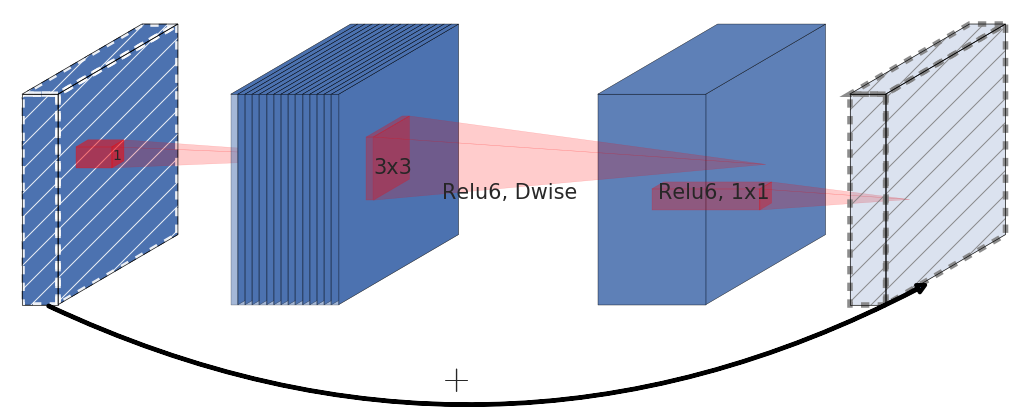
\includegraphics{./figures/inverted_residual.png}}
    \caption{MobileNet V2 Inverted Residual BottleNeck
    Block~\cite[p. 3]{mobile_net_v2_paper}}\label{fig:invertedResidualBottleneckBlock}
\end{figure}

\begin{figure}[H]
    \centering
    \resizebox{\linewidth}{!}{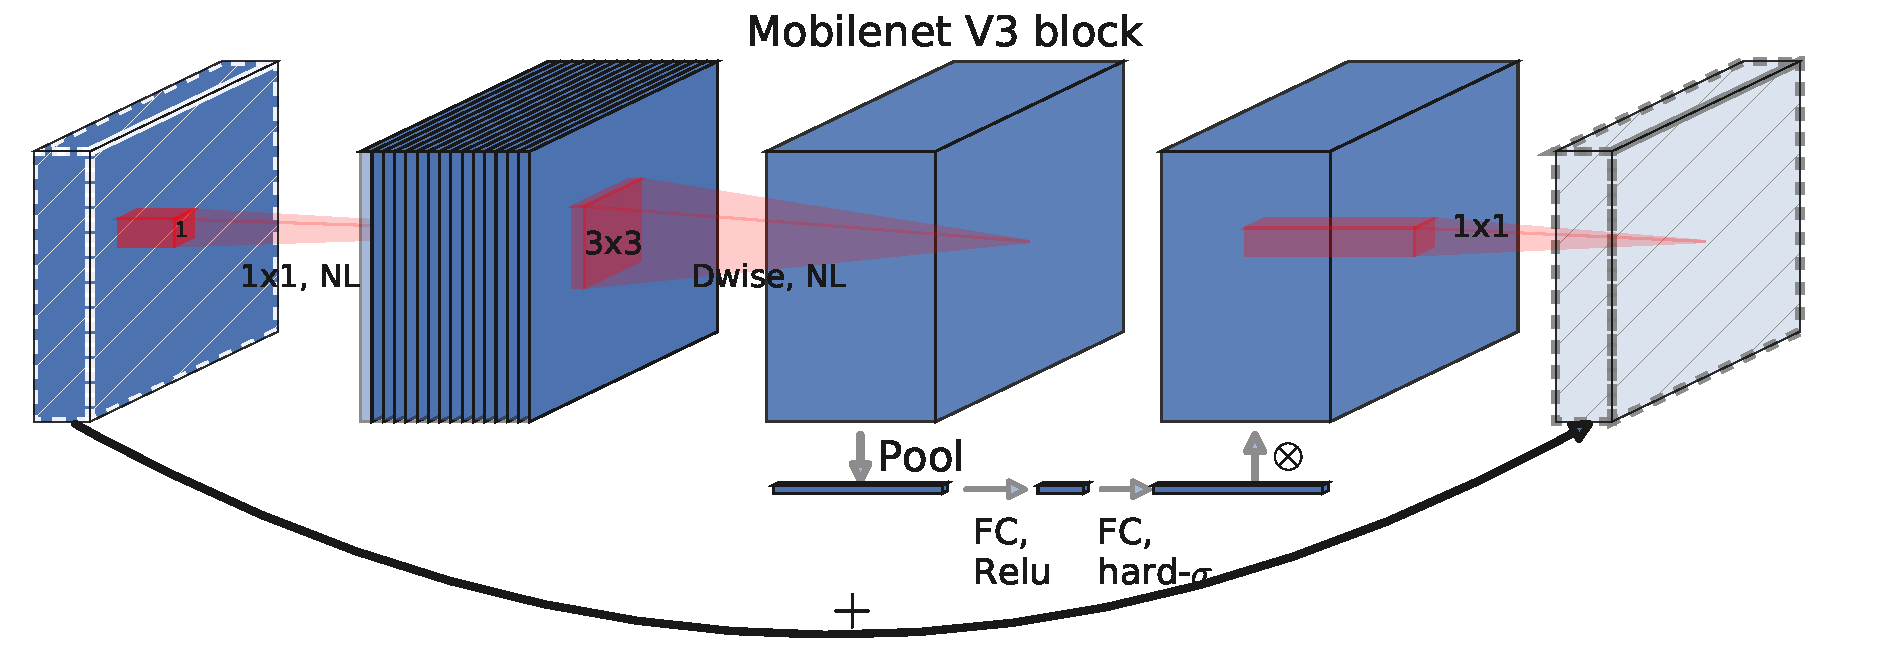
\includegraphics{./figures/mobilenet_v3_block.pdf}}
    \caption{MobileNet V3 Inverted Residual BottleNeck
    Block~\cite{mobile_net_v3_paper}}\label{fig:mobilenet_v3_block}
\end{figure}


\begin{table}[H]
    \centering
    \resizebox{\linewidth}{!}{\begin{tabular}{@{}ccccccc@{}}
        \toprule
        & \multicolumn{2}{c}{Input Dimensions} \\
        \cmidrule{2-3}
        Layer  & Channels & Size & \multirow{-2}{10ex}{\centering Expansion
        Factor} & Repeats & Stride & \multirow{-2}{9ex}{\centering Output
        Channels}\\
        \midrule

        Image       & 3 & 28$\times$28 & --- & --- & --- & --- \\
        Convolution & 3 & 28$\times$28 & --- & 1   & 1   & 32  \\

        \bottomrule\smallskip
    \end{tabular}}\caption{MobileNet V2 tail for CIFAR 10
    dataset.}\label{table:MobileNetCifar10TailArchitecture}
\end{table}

\begin{table}[H]
    \centering
    \resizebox{\linewidth}{!}{\begin{tabular}{@{}ccccccc@{}}
        \toprule
        & \multicolumn{2}{c}{Input Dimensions} \\
        \cmidrule{2-3}
        Layer  & Channels & Size & \multirow{-2}{10ex}{\centering Expansion
        Factor} & Repeats & Stride & \multirow{-2}{9ex}{\centering Output
        Channels}\\
        \midrule

        Residual Bottleneck & 32  & 28$\times$28 & 6 & 4 & 2 & 64  \\
        Residual Bottleneck & 64  & 14$\times$14 & 6 & 3 & 1 & 96  \\
        Residual Bottleneck & 96  & 14$\times$14 & 6 & 3 & 2 & 160 \\
        Residual Bottleneck & 160 & 7$\times$7   & 6 & 1 & 1 & 320 \\

        \bottomrule\smallskip
    \end{tabular}}\caption{MobileNet V2 body for MNIST
    dataset.}\label{table:MobileNetCifar10BodyArchitecture}
\end{table}

\begin{table}[H]
    \centering
    \resizebox{\linewidth}{!}{\begin{tabular}{@{}ccccccc@{}}
        \toprule
        & \multicolumn{2}{c}{Input Dimensions} \\
        \cmidrule{2-3}
        Layer  & Channels & Size & \multirow{-2}{10ex}{\centering Expansion
        Factor} & Repeats & Stride & \multirow{-2}{9ex}{\centering Output
        Channels}\\
        \midrule

        Global Average Pool & 320 & 7$\times$7 & --- & 1 & --- & --- \\
        Dense (softmax)     & 1   & 320        & --- & 1 & --- & 10  \\

        \bottomrule\smallskip
    \end{tabular}}\caption{MobileNet V2 head for MNIST Dataset
    dataset.}\label{table:MobileNetMNISTHeadArchitecture}
\end{table}

\begin{figure}[H]
    \centering
    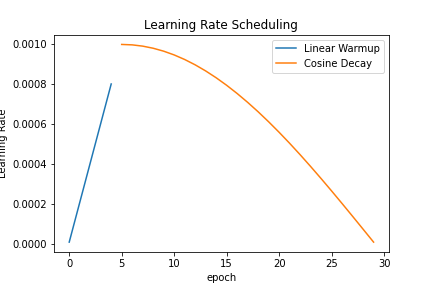
\includegraphics[width=0.8\linewidth]{figures/learning_rate_scheduling.png}
    \caption{Learning Rate Scheduling}\label{fig:learning_rate_scheduling}
\end{figure}


\begin{table}[H]
    \centering
    \resizebox{\linewidth}{!}{\begin{tabular}{@{}ccc@{}}
        \toprule
        & \multicolumn{2}{c}{Hyper Parameters} \\
        \cmidrule{2-3}
            Combination Label & Linear Warmup Epoch Count & Max Learning Rate\\
        \midrule

        1 & 1 & 0.01   \\
        2 & 1 & 0.001  \\
        3 & 1 & 0.0001 \\
        4 & 3 & 0.1    \\
        5 & 3 & 0.001  \\
        6 & 3 & 0.0001 \\
        7 & 5 & 0.1    \\
        8 & 5 & 0.001  \\
        9 & 5 & 0.0001 \\

        \bottomrule\smallskip
    \end{tabular}}\caption{Hyper-Parameter Combinations}\label{table:HyperParamCombinations}
\end{table}


\begin{figure}[H]
    \centering
    \includesvg[width=56ex]{./figures/resnet_v2_train_loss.svg}
    \caption{ResNet 50 --- Log Training Loss vs Epochs}
\end{figure}

\begin{figure}[H]
    \centering
    \includesvg[width=56ex]{./figures/resnet_v2_validation_loss.svg}
    \caption{ResNet 50 --- Log Validation Loss vs Epochs}
\end{figure}


\begin{figure}[H]
    \centering
    \includesvg[width=56ex]{./figures/resnet_v2_validation_loss_no_4.svg}
    \caption{\centering ResNet 50 --- Log Validation Loss vs Epochs Without Combination 4}
\end{figure}


\begin{figure}[H]
    \centering
    \includesvg[width=56ex]{./figures/mobilenet_v2_train_loss.svg}
    \caption{MobileNet V2 --- Log Training Loss vs Epochs}
\end{figure}

\begin{figure}[H]
    \centering
    \includesvg[width=56ex]{./figures/mobilenet_v2_validation_loss.svg}
    \caption{MobileNet V2 --- Log Validation Loss vs Epochs}
\end{figure}


\begin{figure}[H]
    \centering
    \includesvg[width=56ex]{./figures/mobilenet_v3_train_loss.svg}
    \caption{MobileNet V3 --- Log Training Loss vs Epochs}
\end{figure}

\begin{figure}[H]
    \centering
    \includesvg[width=56ex]{./figures/mobilenet_v3_validation_loss.svg}
    \caption{MobileNet V3 --- Log Validation Loss vs Epochs}
\end{figure}


\appendix % {{{

% The following appendix section contains the full tabular results of all
% possible hyperparameter tuning results. Refer to
% Table~\ref{table:HyperParamCombinations} for exact hyper-parameter values.


\subsection{ResNet-50 Detailed Tabular Training Loss Results} % {{{

\begin{table}[H]
    \centering
    \begin{tabular}{@{}cccc@{}}
        \toprule
        & \multicolumn{3}{c}{Hyper Parameter Combination} \\
        \cmidrule{2-4}
            Epoch  & 1 & 2 & 3\\
        \midrule

        0 & 1.62E-06 & 1.78E-06 & 4.33E-07 \\
        1 & 1.56E-04 & 2.82E-06 & 2.46E-06 \\
        2 & 8.99E-05 & 9.91E-07 & 1.70E-07 \\
        3 & 6.57E-05 & 9.63E-07 & 8.63E-08 \\
        4 & 4.66E-05 & 5.71E-07 & 6.09E-08 \\
        5 & 3.64E-05 & 7.69E-07 & 5.11E-08 \\
        6 & 2.57E-05 & 1.08E-07 & 3.88E-08 \\
        7 & 1.58E-05 & 2.07E-07 & 1.76E-08 \\
        8 & 4.78E-06 & 2.88E-06 & 1.68E-07 \\
        9 & 2.50E-06 & 6.21E-08 & 5.29E-07 \\

        \bottomrule\smallskip
    \end{tabular}
    \caption{ResNet V2 Training Loss HyperParameter Combinations 1--3}%
    \label{table:ResNetTrainingLoss1-3}
\end{table}


\begin{table}[H]
    \centering
    \begin{tabular}{@{}cccc@{}}
        \toprule
        & \multicolumn{3}{c}{Hyper Parameter Combination} \\
        \cmidrule{2-4}
            Epoch  & 4 & 5 & 6\\
        \midrule

        0 & 3.61E-08 & 1.29E-06 & 1.18E-07 \\
        1 & 1.64E-05 & 3.71E-06 & 2.85E-07 \\
        2 & 4.30E-05 & 8.91E-07 & 5.82E-08 \\
        3 & 6.23E-05 & 1.55E-06 & 5.86E-08 \\
        4 & 4.40E-05 & 1.10E-06 & 2.24E-07 \\
        5 & 3.56E-05 & 1.49E-06 & 2.63E-07 \\
        6 & 3.74E-05 & 1.78E-07 & 1.28E-07 \\
        7 & 5.50E-06 & 5.15E-07 & 1.84E-07 \\
        8 & 3.14E-06 & 1.22E-07 & 5.21E-08 \\
        9 & 1.12E-06 & 8.19E-08 & 4.98E-08 \\

        \bottomrule\smallskip
    \end{tabular}
    \caption{ResNet V2 Training Loss HyperParameter Combinations 4--6}%
    \label{table:ResNetTrainingLoss4-6}
\end{table}


\begin{table}[H]
    \centering
    \begin{tabular}{@{}cccc@{}}
        \toprule
        & \multicolumn{3}{c}{Hyper Parameter Combination} \\
        \cmidrule{2-4}
            Epoch  & 7 & 8 & 9\\
        \midrule

        0 & 3.45E-07 & 6.93E-07 & 2.52E-08 \\
        1 & 5.01E-08 & 8.03E-07 & 7.51E-07 \\
        2 & 8.90E-06 & 1.82E-06 & 2.47E-08 \\
        3 & 3.54E-05 & 4.40E-06 & 8.56E-08 \\
        4 & 1.70E-05 & 2.22E-07 & 2.52E-07 \\
        5 & 2.64E-05 & 1.77E-06 & 9.32E-08 \\
        6 & 3.65E-05 & 4.50E-07 & 1.70E-07 \\
        7 & 2.23E-05 & 2.37E-07 & 3.86E-08 \\
        8 & 5.42E-06 & 7.97E-08 & 1.96E-08 \\
        9 & 1.36E-06 & 7.55E-08 & 3.32E-08 \\

        \bottomrule\smallskip
    \end{tabular}
    \caption{ResNet V2 Training Loss HyperParameter Combinations 7--9}%
    \label{table:ResNetTrainingLoss7-9}
\end{table}

% }}}


\subsection{ResNet-50 Detailed Tabular Validation Loss Results} % {{{

\begin{table}[H]
    \centering
    \begin{tabular}{@{}cccc@{}}
        \toprule
        & \multicolumn{3}{c}{Hyper Parameter Combination} \\
        \cmidrule{2-4}
            Epoch  & 1 & 2 & 3\\
        \midrule

        0 & 8.02E-05 & 8.56E-05 & 2.35E-04 \\
        1 & 1.81E-04 & 9.92E-05 & 1.84E-04 \\
        2 & 2.22E-03 & 7.07E-05 & 1.96E-04 \\
        3 & 2.92E-05 & 3.81E-04 & 6.47E-05 \\
        4 & 1.64E-04 & 7.26E-05 & 8.81E-05 \\
        5 & 1.33E-04 & 2.26E-05 & 3.78E-05 \\
        6 & 1.79E-04 & 1.22E-04 & 3.63E-05 \\
        7 & 4.15E-03 & 3.96E-06 & 9.13E-05 \\
        8 & 2.75E-04 & 9.87E-05 & 4.68E-05 \\
        9 & 1.40E-04 & 3.13E-05 & 6.55E-05 \\

        \bottomrule\smallskip
    \end{tabular}
    \caption{ResNet V2 Validation Loss HyperParameter Combinations 1--3}%
    \label{table:ResNetValidationLoss1-3}
\end{table}


\begin{table}[H]
    \centering
    \begin{tabular}{@{}cccc@{}}
        \toprule
        & \multicolumn{3}{c}{Hyper Parameter Combination} \\
        \cmidrule{2-4}
            Epoch  & 4 & 5 & 6\\
        \midrule

        0 & 1.09E-04 & 1.78E-04 & 1.24E-04 \\
        1 & 3.64E-05 & 1.00E-04 & 1.37E-05 \\
        2 & 1.83E-01 & 1.33E-04 & 1.53E-04 \\
        3 & 1.96E+00 & 4.19E-04 & 8.80E-05 \\
        4 & 3.13E-05 & 2.39E-04 & 9.33E-05 \\
        5 & 7.62E-01 & 1.14E-04 & 1.21E-04 \\
        6 & 2.54E-03 & 6.70E-05 & 1.95E-04 \\
        7 & 3.91E-04 & 5.55E-05 & 1.40E-04 \\
        8 & 6.78E-04 & 4.09E-05 & 4.83E-04 \\
        9 & 1.38E-04 & 1.81E-04 & 2.04E-04 \\

        \bottomrule\smallskip
    \end{tabular}
    \caption{ResNet V2 Validation Loss HyperParameter Combinations 4--6}%
    \label{table:ResNetValidationLoss4-6}
\end{table}


\begin{table}[H]
    \centering
    \begin{tabular}{@{}cccc@{}}
        \toprule
        & \multicolumn{3}{c}{Hyper Parameter Combination} \\
        \cmidrule{2-4}
            Epoch  & 7 & 8 & 9\\
        \midrule

        0 & 3.50E-04 & 3.98E-04 & 5.19E-04 \\
        1 & 3.36E-04 & 4.65E-04 & 3.59E-04 \\
        2 & 8.12E-06 & 8.41E-04 & 3.90E-04 \\
        3 & 5.12E-04 & 2.76E-04 & 4.84E-04 \\
        4 & 4.18E-05 & 3.92E-04 & 3.60E-04 \\
        5 & 2.28E-04 & 4.22E-04 & 3.25E-04 \\
        6 & 1.89E-05 & 8.59E-04 & 6.15E-04 \\
        7 & 6.85E-04 & 3.49E-04 & 6.74E-04 \\
        8 & 8.36E-05 & 5.76E-04 & 3.47E-04 \\
        9 & 3.23E-04 & 3.32E-04 & 4.35E-04 \\

        \bottomrule\smallskip
    \end{tabular}
    \caption{ResNet V2 Validation Loss HyperParameter Combinations 7--9}%
    \label{table:ResNetValidationLoss7-9}
\end{table}

% }}}


\subsection{MobileNet V2 Detailed Tabular Training Loss Results} % {{{

\begin{table}[H]
    \centering
    \begin{tabular}{@{}cccc@{}}
        \toprule
        & \multicolumn{3}{c}{Hyper Parameter Combination} \\
        \cmidrule{2-4}
            Epoch  & 1 & 2 & 3\\
        \midrule

        0 & 3.40E-04 & 1.99E-03 & 2.46E-06 \\
        1 & 5.97E-04 & 2.09E-04 & 2.61E-06 \\
        2 & 2.47E-04 & 1.53E-04 & 8.01E-07 \\
        3 & 1.86E-04 & 7.98E-05 & 1.38E-07 \\
        4 & 1.14E-04 & 7.40E-05 & 4.27E-08 \\
        5 & 1.04E-04 & 3.77E-05 & 2.06E-07 \\
        6 & 8.76E-05 & 2.24E-05 & 1.22E-06 \\
        7 & 3.19E-05 & 9.36E-06 & 9.36E-08 \\
        8 & 2.46E-05 & 3.62E-06 & 3.25E-08 \\
        9 & 9.67E-06 & 2.30E-06 & 2.87E-06 \\

        \bottomrule\smallskip
    \end{tabular}
    \caption{MobileNet V2 Training Loss HyperParameter Combinations 1--3}%
    \label{table:MobileNetV2TrainingLoss1-3}
\end{table}


\begin{table}[H]
    \centering
    \begin{tabular}{@{}cccc@{}}
        \toprule
        & \multicolumn{3}{c}{Hyper Parameter Combination} \\
        \cmidrule{2-4}
            Epoch  & 4 & 5 & 6\\
        \midrule

        0 & 1.51E-06 & 5.60E-06 & 1.13E-06 \\
        1 & 2.31E-04 & 7.04E-06 & 1.64E-07 \\
        2 & 2.37E-04 & 2.84E-06 & 3.33E-07 \\
        3 & 2.76E-04 & 1.86E-06 & 9.69E-08 \\
        4 & 1.39E-04 & 5.85E-07 & 1.09E-06 \\
        5 & 7.73E-05 & 1.04E-06 & 2.44E-07 \\
        6 & 6.10E-05 & 2.51E-06 & 8.82E-07 \\
        7 & 4.71E-05 & 2.69E-07 & 1.50E-07 \\
        8 & 1.28E-05 & 3.45E-07 & 1.68E-07 \\
        9 & 6.63E-06 & 1.72E-06 & 2.80E-07 \\

        \bottomrule\smallskip
    \end{tabular}
    \caption{MobileNet V2 Training Loss HyperParameter Combinations 4--6}%
    \label{table:MobileNetV2TrainingLoss4-6}
\end{table}


\begin{table}[H]
    \centering
    \begin{tabular}{@{}cccc@{}}
        \toprule
        & \multicolumn{3}{c}{Hyper Parameter Combination} \\
        \cmidrule{2-4}
            Epoch  & 7 & 8 & 9\\
        \midrule

        0 & 1.30E-07 & 4.21E-06 & 6.07E-07 \\
        1 & 2.13E-06 & 3.87E-06 & 8.36E-07 \\
        2 & 3.25E-05 & 4.34E-06 & 2.95E-07 \\
        3 & 6.01E-05 & 1.08E-06 & 9.23E-07 \\
        4 & 5.91E-05 & 5.32E-06 & 7.39E-07 \\
        5 & 7.13E-05 & 9.79E-07 & 2.31E-07 \\
        6 & 8.75E-05 & 3.89E-06 & 8.10E-07 \\
        7 & 2.38E-05 & 3.83E-07 & 5.33E-07 \\
        8 & 1.70E-05 & 5.30E-07 & 3.35E-07 \\
        9 & 3.55E-06 & 4.34E-07 & 1.09E-06 \\

        \bottomrule\smallskip
    \end{tabular}
    \caption{MobileNet V2 Training Loss HyperParameter Combinations 7--9}%
    \label{table:MobileNetV2TrainingLoss7-9}
\end{table}

% }}}


\subsection{MobileNet V2 Detailed Tabular Validation Loss Results} % {{{

\begin{table}[H]
    \centering
    \begin{tabular}{@{}cccc@{}}
        \toprule
        & \multicolumn{3}{c}{Hyper Parameter Combination} \\
        \cmidrule{2-4}
            Epoch  & 1 & 2 & 3\\
        \midrule

        0 & 4.62E-03 & 5.76E-04 & 3.80E-02 \\
        1 & 3.26E-02 & 9.22E-04 & 6.36E-02 \\
        2 & 7.43E-03 & 1.43E-04 & 5.89E-02 \\
        3 & 7.56E-03 & 2.35E-03 & 3.03E-02 \\
        4 & 1.52E-02 & 3.33E-02 & 3.05E-02 \\
        5 & 5.48E-03 & 5.06E-03 & 2.99E-02 \\
        6 & 1.63E-02 & 2.50E-03 & 3.54E-02 \\
        7 & 1.17E-02 & 4.51E-03 & 3.15E-02 \\
        8 & 7.38E-03 & 6.23E-03 & 4.87E-02 \\
        9 & 1.29E-02 & 1.25E-02 & 5.00E-02 \\

        \bottomrule\smallskip
    \end{tabular}
    \caption{MobileNet V2 Validation Loss HyperParameter Combinations 1--3}%
    \label{table:MobileNetV2ValidationLoss1-3}
\end{table}


\begin{table}[H]
    \centering
    \begin{tabular}{@{}cccc@{}}
        \toprule
        & \multicolumn{3}{c}{Hyper Parameter Combination} \\
        \cmidrule{2-4}
            Epoch  & 4 & 5 & 6\\
        \midrule

        0 & 8.54E-02 & 1.98E-02 & 1.77E-02 \\
        1 & 9.60E-03 & 1.88E-02 & 2.32E-02 \\
        2 & 5.88E-03 & 1.98E-02 & 2.38E-02 \\
        3 & 4.63E-02 & 2.04E-02 & 2.56E-02 \\
        4 & 9.32E-03 & 1.91E-02 & 2.58E-02 \\
        5 & 1.35E-02 & 1.95E-02 & 3.04E-02 \\
        6 & 4.72E-01 & 1.72E-02 & 2.66E-02 \\
        7 & 1.88E-02 & 3.72E-02 & 2.19E-02 \\
        8 & 1.51E-02 & 2.31E-02 & 2.30E-02 \\
        9 & 1.87E-02 & 2.37E-02 & 2.55E-02 \\

        \bottomrule\smallskip
    \end{tabular}
    \caption{MobileNet V2 Validation Loss HyperParameter Combinations 4--6}%
    \label{table:MobileNetV2ValidationLoss4-6}
\end{table}


\begin{table}[H]
    \centering
    \begin{tabular}{@{}cccc@{}}
        \toprule
        & \multicolumn{3}{c}{Hyper Parameter Combination} \\
        \cmidrule{2-4}
            Epoch  & 7 & 8 & 9\\
        \midrule

        0 & 3.10E-02 & 2.39E-02 & 3.68E-02 \\
        1 & 1.12E-01 & 3.50E-02 & 3.25E-02 \\
        2 & 3.95E-02 & 2.85E-02 & 4.58E-02 \\
        3 & 3.07E-02 & 3.03E-02 & 4.12E-02 \\
        4 & 1.47E-02 & 4.45E-02 & 3.02E-02 \\
        5 & 9.51E-03 & 4.36E-02 & 3.80E-02 \\
        6 & 3.84E-02 & 3.16E-02 & 3.85E-02 \\
        7 & 3.98E-02 & 4.11E-02 & 3.91E-02 \\
        8 & 2.57E-02 & 3.78E-02 & 3.98E-02 \\
        9 & 3.49E-02 & 3.95E-02 & 3.67E-02 \\

        \bottomrule\smallskip
    \end{tabular}
    \caption{MobileNet V2 Validation Loss HyperParameter Combinations 7--9}%
    \label{table:MobileNetV2ValidationLoss7-9}
\end{table}

% }}}


\subsection{MobileNet V3 Detailed Tabular Training Loss Results} % {{{

\begin{table}[H]
    \centering
    \begin{tabular}{@{}cccc@{}}
        \toprule
        & \multicolumn{3}{c}{Hyper Parameter Combination} \\
        \cmidrule{2-4}
            Epoch  & 1 & 2 & 3\\
        \midrule

        0 & 1.89E-03 & 2.36E-05 & 4.87E-07 \\
        1 & 1.45E-02 & 3.22E-05 & 1.05E-06 \\
        2 & 2.26E-03 & 1.31E-05 & 1.59E-06 \\
        3 & 7.02E-04 & 1.12E-05 & 4.24E-07 \\
        4 & 6.09E-04 & 8.53E-06 & 1.37E-06 \\
        5 & 3.99E-04 & 1.52E-05 & 1.77E-07 \\
        6 & 2.79E-04 & 1.92E-06 & 4.23E-08 \\
        7 & 1.40E-04 & 5.81E-06 & 6.93E-06 \\
        8 & 5.19E-05 & 2.36E-06 & 1.16E-07 \\
        9 & 4.44E-05 & 1.77E-06 & 1.36E-05 \\

        \bottomrule\smallskip
    \end{tabular}
    \caption{MobileNet V3 Training Loss HyperParameter Combinations 1--3}%
    \label{table:MobileNetV3TrainingLoss1-3}
\end{table}


\begin{table}[H]
    \centering
    \begin{tabular}{@{}cccc@{}}
        \toprule
        & \multicolumn{3}{c}{Hyper Parameter Combination} \\
        \cmidrule{2-4}
            Epoch  & 4 & 5 & 6\\
        \midrule

        0 & 7.84E-06 & 1.74E-05 & 5.81E-06 \\
        1 & 2.45E-04 & 1.38E-05 & 2.40E-06 \\
        2 & 2.53E-04 & 8.57E-06 & 9.13E-07 \\
        3 & 1.06E-03 & 2.71E-05 & 1.24E-06 \\
        4 & 4.30E-04 & 6.41E-06 & 8.21E-07 \\
        5 & 5.63E-04 & 1.12E-05 & 4.00E-06 \\
        6 & 3.09E-04 & 7.80E-06 & 1.02E-06 \\
        7 & 1.13E-04 & 3.77E-06 & 1.46E-06 \\
        8 & 7.16E-05 & 4.23E-06 & 6.61E-07 \\
        9 & 3.75E-05 & 2.63E-06 & 1.59E-06 \\

        \bottomrule\smallskip
    \end{tabular}
    \caption{MobileNet V3 Training Loss HyperParameter Combinations 4--6}%
    \label{table:MobileNetV3TrainingLoss4-6}
\end{table}


\begin{table}[H]
    \centering
    \begin{tabular}{@{}cccc@{}}
        \toprule
        & \multicolumn{3}{c}{Hyper Parameter Combination} \\
        \cmidrule{2-4}
            Epoch  & 7 & 8 & 9\\
        \midrule

        0 & 2.08E-06 & 2.78E-05 & 6.14E-05 \\
        1 & 3.81E-05 & 2.34E-05 & 2.87E-06 \\
        2 & 7.35E-05 & 1.36E-05 & 5.93E-06 \\
        3 & 2.40E-04 & 1.08E-05 & 2.14E-06 \\
        4 & 4.01E-04 & 1.18E-05 & 1.12E-06 \\
        5 & 4.08E-04 & 3.13E-05 & 3.59E-06 \\
        6 & 4.01E-04 & 1.02E-05 & 7.57E-07 \\
        7 & 1.38E-04 & 2.93E-06 & 9.77E-08 \\
        8 & 8.24E-05 & 8.84E-06 & 6.54E-07 \\
        9 & 3.79E-05 & 2.31E-06 & 8.65E-07 \\

        \bottomrule\smallskip
    \end{tabular}
    \caption{MobileNet V3 Training Loss HyperParameter Combinations 7--9}%
    \label{table:MobileNetV3TrainingLoss7-9}
\end{table}

% }}}


\subsection{MobileNet V3 Detailed Tabular Validation Loss Results} % {{{

\begin{table}[H]
    \centering
    \begin{tabular}{@{}cccc@{}}
        \toprule
        & \multicolumn{3}{c}{Hyper Parameter Combination} \\
        \cmidrule{2-4}
            Epoch  & 1 & 2 & 3\\
        \midrule

        0 & 2.41E-03 & 3.33E-05 & 1.26E-05 \\
        1 & 3.21E-03 & 1.44E-05 & 4.27E-06 \\
        2 & 4.00E-04 & 3.12E-05 & 2.35E-05 \\
        3 & 1.67E-04 & 1.38E-05 & 1.47E-05 \\
        4 & 2.60E-04 & 1.42E-05 & 7.14E-06 \\
        5 & 1.39E-04 & 1.60E-05 & 5.60E-06 \\
        6 & 6.89E-04 & 2.67E-05 & 7.56E-06 \\
        7 & 1.13E-04 & 4.78E-06 & 7.09E-06 \\
        8 & 1.27E-04 & 7.05E-06 & 6.20E-06 \\
        9 & 2.92E-05 & 1.21E-05 & 4.07E-06 \\

        \bottomrule\smallskip
    \end{tabular}
    \caption{MobileNet V3 Validation Loss HyperParameter Combinations 1--3}%
    \label{table:MobileNetV3ValidationLoss1-3}
\end{table}


\begin{table}[H]
    \centering
    \begin{tabular}{@{}cccc@{}}
        \toprule
        & \multicolumn{3}{c}{Hyper Parameter Combination} \\
        \cmidrule{2-4}
            Epoch  & 4 & 5 & 6\\
        \midrule

        0 & 2.80E-05 & 2.80E-05 & 1.04E-04 \\
        1 & 1.75E-04 & 1.75E-04 & 9.05E-05 \\
        2 & 5.10E-04 & 5.10E-04 & 8.73E-05 \\
        3 & 3.08E-04 & 3.08E-04 & 4.65E-05 \\
        4 & 2.70E-03 & 2.70E-03 & 8.43E-05 \\
        5 & 1.31E-04 & 1.31E-04 & 8.42E-05 \\
        6 & 1.02E-04 & 1.02E-04 & 6.92E-05 \\
        7 & 1.11E-04 & 1.11E-04 & 7.09E-05 \\
        8 & 3.25E-05 & 3.25E-05 & 6.58E-05 \\
        9 & 2.61E-05 & 2.61E-05 & 7.28E-05 \\

        \bottomrule\smallskip
    \end{tabular}
    \caption{MobileNet V3 Validation Loss HyperParameter Combinations 4--6}%
    \label{table:MobileNetV3ValidationLoss4-6}
\end{table}


\begin{table}[H]
    \centering
    \begin{tabular}{@{}cccc@{}}
        \toprule
        & \multicolumn{3}{c}{Hyper Parameter Combination} \\
        \cmidrule{2-4}
            Epoch  & 7 & 8 & 9\\
        \midrule

        0 & 7.10E-05 & 1.68E-04 & 1.55E-04 \\
        1 & 2.89E-04 & 1.47E-04 & 1.65E-04 \\
        2 & 4.55E-05 & 4.05E-04 & 1.49E-04 \\
        3 & 1.28E-04 & 3.78E-04 & 1.57E-04 \\
        4 & 8.93E-05 & 1.90E-04 & 1.42E-04 \\
        5 & 7.47E-03 & 1.75E-04 & 2.10E-04 \\
        6 & 4.93E-04 & 2.18E-04 & 2.48E-04 \\
        7 & 7.00E-04 & 2.35E-04 & 2.31E-04 \\
        8 & 1.53E-04 & 1.68E-04 & 2.56E-04 \\
        9 & 2.37E-04 & 1.42E-04 & 2.86E-04 \\

        \bottomrule\smallskip
    \end{tabular}
    \caption{MobileNet V3 Validation Loss HyperParameter Combinations 7--9}%
    \label{table:MobileNetV3ValidationLoss7-9}
\end{table}

% }}}


% }}}

\end{document}
